\documentclass{report}
\usepackage{graphicx}
\usepackage{fancyhdr}
\usepackage{float}
\usepackage[hidelinks]{hyperref}
\usepackage{letterspace}
\usepackage{xcolor}
\usepackage{pagecolor}
\usepackage[a4paper, hmargin=1.2in, bottom=1.2in]{geometry}
\usepackage{fontspec}
\usepackage{amsmath}
\usepackage{eso-pic}
\usepackage{titlesec}
\usepackage{setspace}
\usepackage{tikz}
\usepackage{enumitem}

\setlist[itemize,1]{label=\small$\bullet$}
\titleformat{\section}{\fontsize{20}{16}\bfseries}{\thesection}{1em}{}
\setstretch{0.9}
\setmainfont{Rajdhani}[
    BoldFont = Rajdhani Semibold
]

\definecolor{grey}{RGB}{40, 40, 40}
\definecolor{section_color}{RGB}{0, 45, 98}
\definecolor{subsection_color}{RGB}{0, 48, 143}
\definecolor{subsubsection_color}{RGB}{0, 0, 255}
\definecolor{text_color}{RGB}{50, 50, 50}
\definecolor{bgcolor}{RGB}{240, 240, 240}

\begin{document}

\begin{titlepage}

    \pagecolor{bgcolor}
    \begin{center}

        
\includegraphics[width=0.7\textwidth]{iitb_logo.png}

        \vspace{100pt}

        \makebox[\textwidth][c]{%
            {\fontfamily{lmdh}\selectfont \fontsize{35}{45}\selectfont
                    \textcolor{section_color}{\textls[40]{Assignment: 01}}}
        }
        \
        \vspace{10pt}

        \makebox[\textwidth][c]{{\selectfont \fontsize{17}{10}\selectfont
                    \textcolor{grey}{{Design And Analysis of Algorithms}}}}

        \vfill

        {\fontsize{16}{30}\selectfont {\textcolor{grey}{Mradul Sonkar |
                    23B0980}}}
        \\[1.5mm]
        {\fontsize{16}{30}\selectfont {\textcolor{grey}{Instructor: Rohit
                Gurjar}}}

    \end{center}

    \newpage

    \nopagecolor\

    \section*{Algorithm Overview:}
    \vspace{1.0em}

    {\fontsize{12}{18} \selectfont
        The algorithm constructs a Minimum Spanning Tree using Kruksal's
        algorithm. It then tries to reduce the number of red edges while
        keeping
        the
        total weight of the tree under the threshold T.
        The key steps involved in the algorithm are as follows:
        \begin{enumerate}

            \item \textbf{Formation of MST using Kruksal's Algorithm}
                  \begin{itemize}
                      \item We sort edges in ascending order of weight. In case
                            of a
                            tie, ew prefer the edge with blue color.
                      \item I am using a combination of \underbar{DisjointSet}
                            data
                            structure and a \underbar{vector of edges} present
                            in
                            MST.
                  \end{itemize}

            \item \textbf{Optimizing MST by Swapping Edges}
                  \begin{itemize}
                      \item We identify blue edges currently not in the MST,
                            we
                            recognize the cycles that would be formed on their
                            addition.
                      \item We then try to find the heaviest red edge present
                            in
                            the
                            cycle and then swap it with the blue edge.
                      \item We repeat until the weight of the MST becomes less
                            than
                            threshold ($\le T$) or no more such swaps are
                            possible, in case of which we
                            output an error message.
                  \end{itemize}

            \item \textbf{Efficiency Enhancements}
                  \begin{itemize}
                      \item LCA (Lowest Common Ancestor) + Binary Lifting is
                            used
                            to efficiently find the heaviest red edge in the
                            cycle.
                  \end{itemize}

                  \textbf{Time Complexity Analysis}
                  \begin{itemize}
                      \item Constructing the Initial MST $\Longrightarrow$
                            $O(ElogE)$
                            \\({\fontsize{11}{16} \selectfont Complexity of
                                    sorting edges and using Kruskal's
                                    algorithm with Union-Find})
                      \item Reducing MST Cost (Edge Replacement)
                            $\Longrightarrow$ $O(ElogV)$
                            \\ ({\fontsize{11}{16} \selectfont Checking all
                                    edges
                                    outside the MST and trying
                                    to replace the heaviest edge in MST using
                                    LCA
                                    with
                                    binary lifting.})
                      \item \textbf{Overall Complexity}
                            \begin{center}
                                $O(ElogE+ElogV)$
                            \end{center}
                  \end{itemize}
        \end{enumerate}
    }

    \newpage

    \section*{Code Overview:}
    \vspace{1.0em}

    \begin{enumerate}[label={\fontsize{14}{16}\selectfont \arabic*.}]

        \item {\fontsize{14}{16} \selectfont \underbar{Structures Used: }}

              \begin{enumerate}

                  \item {\fontsize{13}{14} \selectfont Edge}

                        \begin{itemize}

                            \fontsize{12}{14} \selectfont

                            \item To store information regarding an edge: start
                                  point
                                  (u), end point (v), weight (w), color (c).

                        \end{itemize}

                        \vspace{0.8em}

                  \item {\fontsize{13}{14} \selectfont Graph}
                        \begin{itemize}

                            \fontsize{12}{14} \selectfont

                            \item To represent a graph, has number of vertices
                                  (V) and edges (E).
                            \item Also a function to insert an edge in the
                                  graph and a list of all edges.

                        \end{itemize}

                        \vspace{0.8em}

                  \item {\fontsize{13}{14} \selectfont Disjoint Set}
                        \begin{itemize}

                            \fontsize{12}{14} \selectfont

                            \item To track the connected components of the
                                  graph as we insert edges to form a MST.
                            \item Has function to find the root of the
                                  connected component and to perform the union
                                  of two sets.

                        \end{itemize}

              \end{enumerate}

              \vspace{0.8em}
        \item {\fontsize{14}{16} \selectfont \underbar{Functions Used: }}

              \begin{enumerate}

                  \item {\fontsize{13}{14} \selectfont formMSTEdges}

                        \begin{itemize}

                            \fontsize{12}{14} \selectfont

                            \item This function just makes a MST for the given
                                  graph.
                            \item We are using default comparator with an
                                  addition to break ties.
                            \item If the weight of the edges is the same, we
                                  prefer blue edges.

                        \end{itemize}
                        \vspace{0.8em}

                  \item {\fontsize{13}{14} \selectfont getResFromMST}

                        \begin{itemize}

                            \fontsize{12}{14} \selectfont

                            \item This function extracts the number of red
                                  edges and the cost of the MST, given the edge
                                  list of a MST.

                        \end{itemize}
                        \vspace{0.8em}

                  \item {\fontsize{13}{14} \selectfont dfs}

                        \begin{itemize}

                            \fontsize{12}{14} \selectfont

                            \item Set up ancestor information, stores the
                                  direct parent of each node.
                            \item Store the maximum weight edge on the path
                                  from the node to its parent.
                            \item Calculate depth of each node.

                        \end{itemize}
                        \vspace{0.8em}

                  \item {\fontsize{13}{14} \selectfont getMaxRedEdge}

                        \begin{itemize}

                            \fontsize{12}{14} \selectfont

                            \item This function finds the maximum weight red
                                  edge in the path between the nodes $u$ and
                                  $v$ in a tree using binary lifting.

                        \end{itemize}
                        \vspace{0.8em}

                  \item {\fontsize{13}{14} \selectfont findAllBlueSwaps}

                        \begin{itemize}
                            \fontsize{12}{14} \selectfont
                            \item This function returns the list of all
                                  candidate blue edges that can be swapped with
                                  the red edges.

                        \end{itemize}
                        \vspace{0.8em}

                  \item {\fontsize{13}{14} \selectfont doSwap}

                        \begin{itemize}
                            \fontsize{12}{14} \selectfont
                            \item This function swaps the red edge with the
                                  blue edge, and modify the total weight and
                                  count of red edges in the MST.

                        \end{itemize}
                        \vspace{0.8em}
              \end{enumerate}

              \newpage

        \item {\fontsize{14}{16} \selectfont \underbar{Additional Points:}}

              \begin{enumerate}

                  \item I have used some macros to simplify my work. They are
                        defined at the top of the code, and precisely are the
                        following:
                        \begin{center}
                            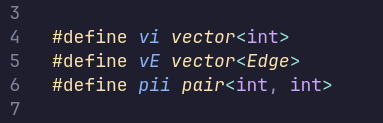
\includegraphics[width = 0.4\textwidth]{image1.png}
                        \end{center}

                  \item I have used fast IO optimization for taking inputs and
                        outputting results faster.
                        \begin{center}
                            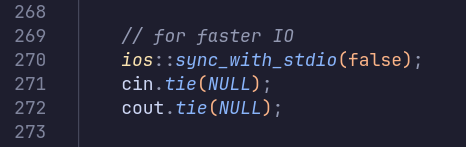
\includegraphics[width = 0.4\textwidth]{image2.png}
                        \end{center}
              \end{enumerate}

              \vspace{0.8em}
        \item {\fontsize{14}{16} \selectfont \underbar{Compilation
                  Steps:}}

              \begin{enumerate}

                  \item The code can be simply compiled using g++ compiler:
                        \begin{verbatim}
                            g++ 23B0980.cpp -o exec
                        \end{verbatim}
                        and can be exectuted in the following way:
                        \begin{verbatim}
                            ./exec
                        \end{verbatim}
                  \item The executable asks for input from user and displays
                        the
                        result.

              \end{enumerate}

              \vspace{0.8em}

        \item {\fontsize{14}{16} \selectfont \underbar{References:}}

              \begin{enumerate}

                  \item

                        \href{https://www.cse.iitb.ac.in/~akg/courses/2024-ds/}{Lecture Slides of
                            course CS213 by Prof. Ashutosh Gupta}

                  \item

                        \href{https://codeforces.com/blog/entry/100826}{Codeforces Tutorial on
                            Binary Lifting}

                  \item

                        \href{https://www.geeksforgeeks.org/lca-in-a-tree-using-binary-lifting-technique/}{
                            LCA in a tree using Binary Lifting Technique
                        } -
                        {\fontsize{9}{15} \selectfont My implementation is
                        inspired by the code available on
                        this page.}

              \end{enumerate}

    \end{enumerate}

\end{titlepage}

\end{document}